\section{Variables and Storage}

The variables of imperative programs \textit{do not} behave like mathematical variables. (A mathematical variable stands for a fixed but unknown value; there is no implication of change over time.) The variables of functional and logic programs \textit{do} behave like mathematical variables.

In imperative (and object-oriented and concurrent) programming languages, a \textit{\textbf{variable}} is a container for a value, and may be \textit{inspected} and \textit{updated} as often as desired.

To understand how the variables of imperative programs really do behave, we need some notion of \textit{\textbf{storage}}. We use an abstract model of storage that is simple but adequate:
\begin{itemize}
  \item A store is a collection of \textit{\textbf{storage cells}}, each of which has a unique address.
  \item Each storage cell has a current \textit{status}, which is either \textit{allocated} or \textit{unallocated}. Each allocated storage cell has a current \textit{content}, which is either a \textit{storable value} or \textit{undefined}.
\end{itemize}

\begin{figure}[H]
  \centering
  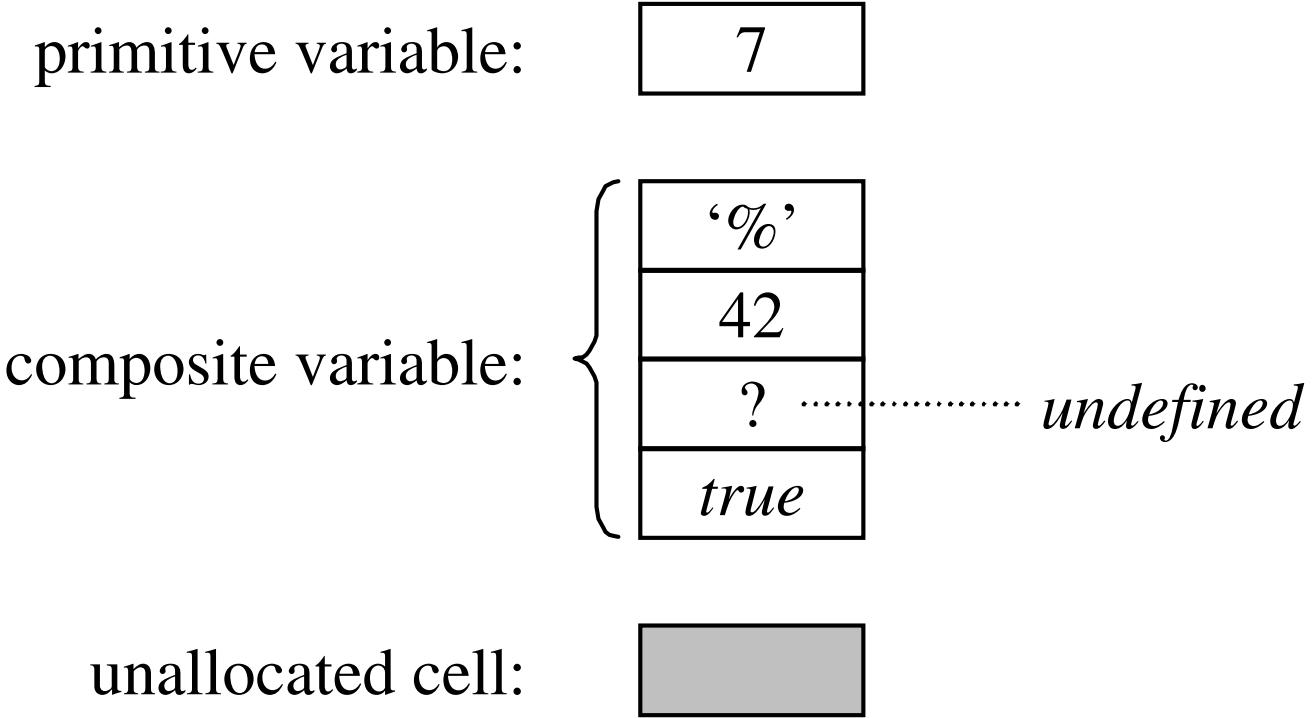
\includegraphics[width=.8\linewidth]{img/fig-3.1.png}
  \caption{An abstract storage model.}
\end{figure}

In terms of this storage model, we can view a variable as a container consisting of one or more storage cells. More precisely:
\begin{itemize}
  \item A \textit{\textbf{simple variable}} occupies a single allocated storage cell.
  \item A \textit{\textbf{composite variable}} occupies a group of contiguous allocated storage cells.
\end{itemize}

A \textit{\textbf{storable}} value is one that can be stored in a single storage cell. Each programming language counts certain types of values as storable:
\begin{itemize}
  \item \texttt{C++}'s storable values are primitive values and pointers. (Structures, arrays, unions, and objects are not storable, since none of these can be stored in a single storage cell. Functions also are not storable, since they cannot be stored at all. However, pointers to all of these things are storable.)
  \item \texttt{JAVA}'s storable values are primitive values and pointers to objects. (Objects themselves are not storable, but every object is implicitly accessed through a pointer.)
\end{itemize}

As a rule of thumb, most programming languages count \textit{primitive values and pointers as storable, but not composite values.}

As an example, in the \hyperref[code:code-1]{code 1}:
\begin{itemize}
  \item When function is called, cells are initially unallocated.
  \item In line 2, cell is allocated/undefined. It is ready to use but value is unknown.
  \item In line 4, it is storable.
  \item In line 6, After the including block terminates, the cell is again unallocated.
\end{itemize}

\begin{listing}[H]
\begin{minted}[linenos, xleftmargin=20pt]{cpp}
void f() {
  int x;
  ...
  x=5;
  ...
  return;
}

f();
\end{minted}
\caption{}
\label{code:code-1}
\end{listing}
